\documentclass{beamer}
% September 2016 
% Author: Dr. Rachid Hourizi and Dr. Michael Wright 
% Department of Computer Science, University of Bath
\usepackage{listings}
\usetheme{Boadilla} 
\lstset{language=C}

\begin{document}

\AtBeginSection[]{
  \begin{frame}
  \vfill
  \centering
  \begin{beamercolorbox}[sep=8pt,center,shadow=true,rounded=true]{title}
    \usebeamerfont{title}\insertsectionhead\par%
  \end{beamercolorbox}
  \vfill
  \end{frame}
}

\title{CM 10227/50258: Getting Started With SRPN}
\author{Dr. Rachid Hourizi and Dr. Michael Wright }
\date{\today}
\frame{\titlepage}

\begin{frame}
\frametitle{Introduction}
\begin{itemize}
\item How can you make a start on the first large coursework
\begin{itemize}
\item When you dont know much Java?
\item When you havent previously written a larger piece of code than that required by the lab sheets?
\end{itemize}
\end{itemize}
\end{frame}


\begin{frame}
\frametitle{Read the Specification}
Read the specification for SRPN, which includes but is not limited to:
\begin{itemize}
\item Your task is to write a program, which matches the functionality of SRPN as closely as possible. 
\item Note that this includes not adding or enhancing existing features. 
\item SRPN is a reverse polish notation calculator 
\item with the extra feature that all arithmetic is saturated 
\item i.e. when it reaches the maximum value that can be stored in a variable, 
\item it stays at the maximum rather than wrapping around.
\item Our marking script will be the same but will use different test-cases.
\item The program includes the less obvious features of srpn.
\end{itemize}
\end{frame}

\begin{frame}[fragile]
\frametitle{Understand RPN}
\begin{itemize}
\item Reverse Polish notation (RPN) is a mathematical notation in which every operator follows all of its operands
\end{itemize}
\begin{block}{}
\begin{lstlisting}
5 4 + =

3 2 * 4 4 * + =
\end{lstlisting}
\end{block}
\end{frame}

\begin{frame}[fragile]
\frametitle{Explore Our Code}
\begin{block}{}
\begin{lstlisting}
10 
2
+ 
=

3 3 * 4 4 * + =

etc
\end{lstlisting}
\end{block}
\end{frame}

\begin{frame}
\frametitle{Code Iteratively}
\begin{itemize}
\item Dont try to write a program that satisfies the whole specification immeditately
\item Write a program that satisfies \textbf{some} of the specification, get it working, \textbf{save it} and then add functionality
\end{itemize}
\end{frame}


\begin{frame}
\frametitle{Find a Small Enough SubProblem To Tackle In Version 1}
Find a Small Enough SubProblem To Tackle In Version 1 e.g.
\begin{itemize}
\item Get any Java program working?
\item Get a Program working that prints to the screen without taking user input?
\item Get a program working that prints integers to the screen when they are entered neatly, one per line
\item Get a program working that also recognises the difference between operators and integers
\item Get a program working that also performs operations on integers before printing
\item Think about an edge case
\item Think abut another edge case
\item etc
\end{itemize}
\end{frame}

\begin{frame}
\frametitle{Review Our Discussion of Stacks}
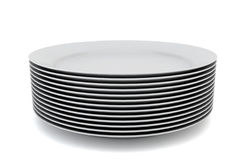
\includegraphics[scale=4.0]{plates.jpg}
\end{frame}

\begin{frame}
\frametitle{Review Our Discussion of Stacks}
\begin{itemize}
\item You might find the concept of a Stack useful when writing SRPN
\item We have seen stacks before
\item Stacks are first in last out (FILO) data structures 
\item i.e. collections of data that give you back the last item that you put in
\bigskip
\item ASIDE: It may be helpful to compare FILO with First In First Out (FIFO) Structures
\item A Queue is a FIFO data structures 
\end{itemize}
\end{frame}

\begin{frame}
\frametitle{Review Our Discussion of Stacks}
\begin{itemize}
\item Stacks provide the following functionality
\bigskip
\begin{itemize}
\item Object push(Object element)
\item Pushes the element onto the stack.
\bigskip
\item boolean empty()
\item Tests whether stack is empty. Returns true if the stack is empty, and returns false if the stack contains elements.
\bigskip
\item Object peek( )
\item Returns the element on the top of the stack, but does not remove it.
\bigskip
\item Object pop( )
\item Returns the element on the top of the stack, removing it in the process.
\bigskip
\end{itemize}
\end{itemize}
\end{frame}

\begin{frame}
\frametitle{Review Our Discussion of Stacks}
\begin{itemize}
\item Java provides a prewritten Stack class
\item i.e. a pre-written template from which you can create Stack Objects
\item http://tinyurl.com/hewobm3f
\bigskip
\item You may use snippets of other people's code
\item but don't forget to provide a reference in comments
\bigskip
\item We dont usually suggest using code that you dont fully understand
\item You may make an exception in this case
\end{itemize}
\end{frame}


\end{document}
